% Generated on 2025-04-15 00:13:35 by gEcon ver. 1.2.1 (2023-01-18)
% http://gecon.r-forge.r-project.org/

% Model name: baseline_NK

\section{Steady-state values}


\begin{tabular}{c|c|}
  & Steady-state value\\
\hline
$\epsilon^{\mathrm{G}}$ & 0.9 \\
$g^{\mathrm{1}}$ & 0.9 \\
$g^{\mathrm{2}}$ & 0.9 \\
$\lambda$ & 0.9 \\
${m\!c}$ & 0.9 \\
$\nu^{\mathrm{p}}$ & 0.9 \\
$\pi$ & 0.9 \\
$\pi^{\star}$ & 0.9 \\
$\pi^{\mathrm{obj}}$ & 0.9 \\
$q$ & 0.9 \\
$r$ & 0.9 \\
$B$ & 0.9 \\
$C$ & 0.9 \\
${D\!i\!v}$ & 0.9 \\
$G$ & 0.9 \\
$I$ & 0.9 \\
$K^{\mathrm{s}}$ & 0.9 \\
$L^{\mathrm{s}}$ & 0.9 \\
$Q$ & 0.9 \\
$R$ & 0.9 \\
$T$ & 0.9 \\
$U$ & 0.9 \\
$W$ & 0.9 \\
$Y$ & 0.9 \\
$Y^{\mathrm{j}}$ & 0.9 \\
$Y^{\mathrm{s}}$ & 0.9 \\
$Z$ & 0.9 \\
\hline
\end{tabular}


\section{The solution of the 1st order perturbation}

\subsection*{Matrix $P$}

$$\bordermatrix{
~ & \epsilon^{\mathrm{G}}_{t-1} & \nu^{\mathrm{p}}_{t-1} & \pi_{t-1} & \pi^{\mathrm{obj}}_{t-1} & B_{t-1} & K^{\mathrm{s}}_{t-1} & R_{t-1} & Z_{t-1} \cr
\epsilon^{\mathrm{G}}_{t} & 0.949 & 0 & 0 & 0 & 0 & 0 & 0 & 0 \cr
\nu^{\mathrm{p}}_{t} & -0.092 & 0.0793 & 0.2373 & -0.6273 & 0 & 0.4827 & 2.8695 & 0.7855 \cr
\pi_{t} & 0.1307 & 0.978 & 0.1319 & 0.8913 & 0 & -0.6858 & -4.0769 & -1.116 \cr
\pi^{\mathrm{obj}}_{t} & 0 & 0 & 0 & 0.924 & 0 & 0 & 0 & 0 \cr
B_{t} & 0 & 0 & 0 & 0 & 0 & 0 & 0 & 0 \cr
K^{\mathrm{s}}_{t} & 0.0856 & 0.2781 & 0.2545 & -0.6491 & 0 & 0.5181 & 1.8624 & -0.3555 \cr
R_{t} & 0.0004 & -0.0003 & 0.0647 & -0.0222 & 0 & -0.0007 & 0.9496 & 0.0002 \cr
Z_{t} & 0 & 0 & 0 & 0 & 0 & 0 & 0 & 0.8385 \cr
}$$

\subsection*{Matrix $Q$}

$$\bordermatrix{
~ & \epsilon^{\mathrm{Z}} & \eta^{\mathrm{p}} & \eta^{\mathrm{R}} & \eta^{\pi} & \eta^{\mathrm{G}} \cr
\epsilon^{\mathrm{G}} & 0 & 0 & 0 & 0 & 1 \cr
\nu^{\mathrm{p}} & 0.9544 & 0.0014 & 2.986 & -0.6789 & -0.0969 \cr
\pi & -1.356 & -0.0021 & -4.2424 & 0.9646 & 0.1377 \cr
\pi^{\mathrm{obj}} & 0 & 0 & 0 & 1 & 0 \cr
B & 0 & 0 & 0 & 0 & 0 \cr
K^{\mathrm{s}} & -0.4319 & 0.0016 & 1.938 & -0.7025 & 0.0902 \cr
R & 0.0002 & 0 & 0.9882 & -0.024 & 0.0004 \cr
Z & 1.0188 & 0 & 0 & 0 & 0 \cr
}$$

\subsection*{Matrix $R$}

$$\bordermatrix{
~ & \epsilon^{\mathrm{G}}_{t-1} & \nu^{\mathrm{p}}_{t-1} & \pi_{t-1} & \pi^{\mathrm{obj}}_{t-1} & B_{t-1} & K^{\mathrm{s}}_{t-1} & R_{t-1} & Z_{t-1} \cr
g^{\mathrm{1}}_{t} & 1.6135 & 9.347 & -4.5292 & 11.5569 & 0 & -6.7553 & -44.3936 & -11.2804 \cr
g^{\mathrm{2}}_{t} & 1.0757 & 6.2313 & -3.0195 & 7.7046 & 0 & -4.5035 & -29.5957 & -7.5203 \cr
\lambda_{t} & 0.191 & 0.9427 & 1.1212 & -2.8972 & 0 & -0.7142 & 10.6339 & -1.0658 \cr
{m\!c}_{t} & 1.5643 & 11.5434 & -2.0392 & 6.665 & 0 & -8.2439 & -35.5872 & -12.8739 \cr
\pi^{\star}_{t} & 0.9342 & 6.9908 & -2.4095 & 6.3709 & 0 & -4.9019 & -29.1422 & -7.9772 \cr
q_{t} & 0.191 & 0.9427 & 1.1212 & -2.8972 & 0 & -0.7142 & 10.6339 & -1.0658 \cr
r_{t} & 0.4224 & 3.1177 & -0.5525 & 1.8047 & 0 & -2.4154 & -9.6296 & -3.2505 \cr
C_{t} & -0.0755 & -0.3539 & -0.4987 & 1.2955 & 0 & 0.2721 & -4.81 & 0.4052 \cr
{D\!i\!v}_{t} & -1.1752 & -9.4305 & 1.4165 & -4.7768 & 0 & 5.5955 & 25.9784 & 9.8026 \cr
G_{t} & 0.0821 & 0 & 0 & 0 & 0 & 0 & 0 & 0 \cr
I_{t} & 0.0856 & 0.2781 & 0.2545 & -0.6491 & 0 & -0.4569 & 1.8624 & -0.3555 \cr
L^{\mathrm{s}}_{t} & 0.0002 & 0.0051 & -0.01 & 0.0273 & 0 & -0.003 & -0.1115 & -0.0047 \cr
Q_{t} & 0 & 0 & 0 & 0 & 0 & 0 & 0 & 0 \cr
T_{t} & -0.0628 & -1.087 & -0.0747 & -1.0149 & 1.1111 & 0.7612 & 5.5851 & 1.2402 \cr
U_{t} & -0.718 & -2.339 & -1.8249 & 5.4146 & 0 & 1.4576 & -14.154 & 3.2399 \cr
W_{t} & 0.9855 & 7.2714 & -1.2828 & 4.1938 & 0 & -5.0041 & -22.3988 & -7.5814 \cr
Y_{t} & 0.0922 & -0.0758 & -0.2443 & 0.6464 & 0 & -0.1848 & -2.9476 & 0.0497 \cr
Y^{\mathrm{j}}_{t} & 0.0002 & 0.0032 & -0.0063 & 0.0172 & 0 & 0.2681 & -0.0703 & 0.7517 \cr
Y^{\mathrm{s}}_{t} & 0.0002 & 0.0032 & -0.0063 & 0.0172 & 0 & 0.2681 & -0.0703 & 0.7517 \cr
}$$

\subsection*{Matrix $S$}

$$\bordermatrix{
~ & \epsilon^{\mathrm{Z}} & \eta^{\mathrm{p}} & \eta^{\mathrm{R}} & \eta^{\pi} & \eta^{\mathrm{G}} \cr
g^{\mathrm{1}} & -13.7064 & -0.0214 & -46.1952 & 12.5074 & 1.7002 \cr
g^{\mathrm{2}} & -9.1376 & -0.755 & -30.7968 & 8.3383 & 1.1335 \cr
\lambda & -1.2951 & -0.0022 & 11.0654 & -3.1355 & 0.2013 \cr
{m\!c} & -15.6427 & -0.9387 & -37.0314 & 7.2132 & 1.6484 \cr
\pi^{\star} & -9.6928 & -0.0147 & -30.3249 & 6.8949 & 0.9844 \cr
q & -1.2951 & -0.0022 & 11.0654 & -3.1355 & 0.2013 \cr
r & -3.9495 & -0.2536 & -10.0204 & 1.9531 & 0.4451 \cr
C & 0.4923 & -0.0037 & -5.0052 & 1.4021 & -0.0796 \cr
{D\!i\!v} & 11.9109 & 0.7591 & 27.0326 & -5.1696 & -1.2383 \cr
G & 0 & 0 & 0 & 0 & 0.0865 \cr
I & -0.4319 & 0.0016 & 1.938 & -0.7025 & 0.0902 \cr
L^{\mathrm{s}} & -0.0057 & -0.0009 & -0.116 & 0.0295 & 0.0003 \cr
Q & 0 & 0 & 0 & 0 & 0 \cr
T & 1.5069 & 0.0023 & 5.8117 & -1.0984 & -0.0661 \cr
U & 3.9367 & 0.0304 & -14.7284 & 5.86 & -0.7566 \cr
W & -9.2119 & -0.5912 & -23.3078 & 4.5387 & 1.0384 \cr
Y & 0.0604 & -0.0021 & -3.0672 & 0.6996 & 0.0971 \cr
Y^{\mathrm{j}} & 0.9133 & -0.0006 & -0.0731 & 0.0186 & 0.0002 \cr
Y^{\mathrm{s}} & 0.9133 & -0.0006 & -0.0731 & 0.0186 & 0.0002 \cr
}$$


\section{Model statistics}

\subsection{Basic statistics}

\begin{tabular}{c|c|c|c|c|}
  & Steady-state value & Std. dev. & Variance & Loglin\\
\hline
$\epsilon^{\mathrm{G}}$ & 0.9 & 1.3033 & 1.6986 & Y    \\
$g^{\mathrm{1}}$ & 0.9 & 48.3192 & 2334.743 & Y    \\
$g^{\mathrm{2}}$ & 0.9 & 32.221 & 1038.1948 & Y    \\
$\lambda$ & 0.9 & 12.7587 & 162.7844 & Y    \\
${m\!c}$ & 0.9 & 39.7072 & 1576.6623 & Y    \\
$\nu^{\mathrm{p}}$ & 0.9 & 4.5824 & 20.9986 & Y    \\
$\pi$ & 0.9 & 5.1772 & 26.8039 & Y    \\
$\pi^{\star}$ & 0.9 & 31.7329 & 1006.9793 & Y    \\
$\pi^{\mathrm{obj}}$ & 0.9 & 1.2958 & 1.6792 & Y    \\
$q$ & 0.9 & 12.7587 & 162.7844 & Y    \\
$r$ & 0.9 & 10.6837 & 114.1408 & Y    \\
$B$ & 0.9 & 0 & 0 & Y    \\
$C$ & 0.9 & 5.7162 & 32.6746 & Y    \\
${D\!i\!v}$ & 0.9 & 30.0911 & 905.4772 & Y    \\
$G$ & 0.9 & 0.1127 & 0.0127 & Y    \\
$I$ & 0.9 & 2.2734 & 5.1681 & Y    \\
$K^{\mathrm{s}}$ & 0.9 & 4.2598 & 18.1462 & Y    \\
$L^{\mathrm{s}}$ & 0.9 & 0.1247 & 0.0155 & Y    \\
$Q$ & 0.9 & 0 & 0 & Y    \\
$R$ & 0.9 & 1.1114 & 1.2353 & Y    \\
$T$ & 0.9 & 6.9169 & 47.843 & Y    \\
$U$ & 0.9 & 18.5085 & 342.5659 & Y    \\
$W$ & 0.9 & 24.9347 & 621.7387 & Y    \\
$Y$ & 0.9 & 3.8656 & 14.9431 & Y    \\
$Y^{\mathrm{j}}$ & 0.9 & 1.5148 & 2.2946 & Y    \\
$Y^{\mathrm{s}}$ & 0.9 & 1.5148 & 2.2946 & Y    \\
$Z$ & 0.9 & 1.2625 & 1.594 & Y    \\
\hline
\end{tabular}


\subsection{Correlation matrix}

\begin{tabular}{c|ccccccccccccccccccccccccc|}
  & $\epsilon^{\mathrm{G}}$ & $g^{\mathrm{1}}$ & $g^{\mathrm{2}}$ & $\lambda$ & ${m\!c}$ & $\nu^{\mathrm{p}}$ & $\pi$ & $\pi^{\star}$ & $\pi^{\mathrm{obj}}$ & $q$ & $r$ & $C$ & ${D\!i\!v}$ & $G$ & $I$ & $K^{\mathrm{s}}$ & $L^{\mathrm{s}}$ & $R$ & $T$ & $U$ & $W$ & $Y$ & $Y^{\mathrm{j}}$ & $Y^{\mathrm{s}}$ & $Z$\\
\hline
$\epsilon^{\mathrm{G}}$ & 1 & 0.012 & 0.012 & 0.019 & 0.009 & -0.009 & 0.006 & 0.004 & 0 & 0.019 & 0.007 & -0.018 & -0.011 & 1 & 0.03 & 0.046 & -0.01 & 0.008 & 0.012 & -0.046 & 0.01 & 0.02 & 0.023 & 0.023 & 0 \\
$g^{\mathrm{1}}$ &  & 1 & 1 & -0.837 & 0.99 & -0.635 & 0.873 & 0.998 & 0.217 & -0.837 & 0.99 & 0.848 & -0.967 & 0.012 & -0.841 & -0.406 & 0.927 & -0.821 & -0.873 & 0.767 & 0.991 & 0.76 & 0.018 & 0.018 & -0.084 \\
$g^{\mathrm{2}}$ &  &  & 1 & -0.837 & 0.991 & -0.635 & 0.873 & 0.998 & 0.217 & -0.837 & 0.99 & 0.848 & -0.967 & 0.012 & -0.841 & -0.406 & 0.927 & -0.821 & -0.872 & 0.766 & 0.992 & 0.76 & 0.018 & 0.018 & -0.084 \\
$\lambda$ &  &  &  & 1 & -0.792 & 0.823 & -0.933 & -0.838 & -0.24 & 1 & -0.82 & -1 & 0.699 & 0.019 & 0.878 & 0.715 & -0.98 & 0.957 & 0.947 & -0.984 & -0.79 & -0.962 & 0.033 & 0.033 & -0.144 \\
${m\!c}$ &  &  &  &  & 1 & -0.625 & 0.87 & 0.995 & 0.139 & -0.792 & 0.996 & 0.804 & -0.98 & 0.009 & -0.786 & -0.367 & 0.897 & -0.808 & -0.867 & 0.704 & 0.999 & 0.728 & -0.031 & -0.031 & -0.158 \\
$\nu^{\mathrm{p}}$ &  &  &  &  &  & 1 & -0.888 & -0.642 & -0.255 & 0.823 & -0.674 & -0.821 & 0.462 & -0.009 & 0.476 & 0.895 & -0.791 & 0.811 & 0.883 & -0.815 & -0.6 & -0.935 & 0.576 & 0.576 & 0.157 \\
$\pi$ &  &  &  &  &  &  & 1 & 0.884 & 0.226 & -0.933 & 0.892 & 0.937 & -0.772 & 0.006 & -0.763 & -0.683 & 0.954 & -0.931 & -0.998 & 0.882 & 0.858 & 0.938 & -0.265 & -0.265 & -0.133 \\
$\pi^{\star}$ &  &  &  &  &  &  &  & 1 & 0.171 & -0.838 & 0.994 & 0.849 & -0.971 & 0.004 & -0.835 & -0.403 & 0.929 & -0.837 & -0.884 & 0.76 & 0.996 & 0.764 & 0.007 & 0.007 & -0.099 \\
$\pi^{\mathrm{obj}}$ &  &  &  &  &  &  &  &  & 1 & -0.24 & 0.157 & 0.238 & -0.091 & 0 & -0.202 & -0.327 & 0.217 & 0.033 & -0.182 & 0.345 & 0.132 & 0.233 & -0.159 & -0.159 & 0 \\
$q$ &  &  &  &  &  &  &  &  &  & 1 & -0.82 & -1 & 0.699 & 0.019 & 0.878 & 0.715 & -0.98 & 0.957 & 0.947 & -0.984 & -0.79 & -0.962 & 0.033 & 0.033 & -0.144 \\
$r$ &  &  &  &  &  &  &  &  &  &  & 1 & 0.832 & -0.962 & 0.007 & -0.779 & -0.44 & 0.916 & -0.831 & -0.89 & 0.741 & 0.994 & 0.773 & -0.06 & -0.06 & -0.118 \\
$C$ &  &  &  &  &  &  &  &  &  &  &  & 1 & -0.714 & -0.018 & -0.881 & -0.707 & 0.984 & -0.958 & -0.951 & 0.981 & 0.803 & 0.96 & -0.031 & -0.031 & 0.136 \\
${D\!i\!v}$ &  &  &  &  &  &  &  &  &  &  &  &  & 1 & -0.011 & 0.786 & 0.182 & -0.825 & 0.722 & 0.771 & -0.598 & -0.985 & -0.594 & -0.106 & -0.106 & 0.163 \\
$G$ &  &  &  &  &  &  &  &  &  &  &  &  &  & 1 & 0.03 & 0.046 & -0.01 & 0.008 & 0.012 & -0.046 & 0.01 & 0.02 & 0.023 & 0.023 & 0 \\
$I$ &  &  &  &  &  &  &  &  &  &  &  &  &  &  & 1 & 0.313 & -0.895 & 0.821 & 0.782 & -0.84 & -0.8 & -0.714 & -0.343 & -0.343 & -0.167 \\
$K^{\mathrm{s}}$ &  &  &  &  &  &  &  &  &  &  &  &  &  &  &  & 1 & -0.63 & 0.651 & 0.685 & -0.776 & -0.346 & -0.86 & 0.463 & 0.463 & -0.204 \\
$L^{\mathrm{s}}$ &  &  &  &  &  &  &  &  &  &  &  &  &  &  &  &  & 1 & -0.954 & -0.964 & 0.94 & 0.896 & 0.929 & -0.02 & -0.02 & 0.062 \\
$R$ &  &  &  &  &  &  &  &  &  &  &  &  &  &  &  &  &  & 1 & 0.953 & -0.901 & -0.805 & -0.934 & 0.063 & 0.063 & -0.071 \\
$T$ &  &  &  &  &  &  &  &  &  &  &  &  &  &  &  &  &  &  & 1 & -0.895 & -0.857 & -0.946 & 0.232 & 0.232 & 0.098 \\
$U$ &  &  &  &  &  &  &  &  &  &  &  &  &  &  &  &  &  &  &  & 1 & 0.702 & 0.956 & -0.023 & -0.023 & 0.245 \\
$W$ &  &  &  &  &  &  &  &  &  &  &  &  &  &  &  &  &  &  &  &  & 1 & 0.717 & 0.011 & 0.011 & -0.131 \\
$Y$ &  &  &  &  &  &  &  &  &  &  &  &  &  &  &  &  &  &  &  &  &  & 1 & -0.248 & -0.248 & 0.103 \\
$Y^{\mathrm{j}}$ &  &  &  &  &  &  &  &  &  &  &  &  &  &  &  &  &  &  &  &  &  &  & 1 & 1 & 0.664 \\
$Y^{\mathrm{s}}$ &  &  &  &  &  &  &  &  &  &  &  &  &  &  &  &  &  &  &  &  &  &  &  & 1 & 0.664 \\
$Z$ &  &  &  &  &  &  &  &  &  &  &  &  &  &  &  &  &  &  &  &  &  &  &  &  & 1 \\
\hline
\end{tabular}


\subsection{Cross correlations with the reference variable ($\pi$)}

\begin{tabular}{c|c|c|c|c|c|c|c|c|c|c|c|c|}
  & $\sigma[\cdot]$ rel. to $\sigma[\pi]$ & $\pi_{t-5}$ & $\pi_{t-4}$ & $\pi_{t-3}$ & $\pi_{t-2}$ & $\pi_{t-1}$ & $\pi_{t}$ & $\pi_{t+1}$ & $\pi_{t+2}$ & $\pi_{t+3}$ & $\pi_{t+4}$ & $\pi_{t+5}$\\
\hline
$\epsilon^{\mathrm{G}}_{t}$ & 0.252 & -0.002 & -0.005 & -0.009 & -0.014 & -0.015 & 0.006 & 0.006 & 0.005 & 0.004 & 0.004 & 0.003 \\
$g^{\mathrm{1}}_{t}$ & 9.333 & -0.095 & -0.044 & 0.054 & 0.224 & 0.496 & 0.873 & 0.037 & -0.06 & -0.1 & -0.115 & -0.118 \\
$g^{\mathrm{2}}_{t}$ & 6.224 & -0.095 & -0.044 & 0.054 & 0.224 & 0.496 & 0.873 & 0.037 & -0.06 & -0.1 & -0.115 & -0.118 \\
$\lambda_{t}$ & 2.464 & 0.159 & 0.1 & -0.017 & -0.221 & -0.539 & -0.933 & -0.459 & -0.168 & 0.003 & 0.098 & 0.147 \\
${m\!c}_{t}$ & 7.67 & -0.088 & -0.04 & 0.051 & 0.213 & 0.478 & 0.87 & 0.035 & -0.07 & -0.114 & -0.129 & -0.128 \\
$\nu^{\mathrm{p}}_{t}$ & 0.885 & 0.273 & 0.239 & 0.146 & -0.042 & -0.372 & -0.888 & -0.72 & -0.511 & -0.317 & -0.155 & -0.03 \\
$\pi_{t}$ & 1 & -0.166 & -0.114 & -0.006 & 0.19 & 0.517 & 1 & 0.517 & 0.19 & -0.006 & -0.114 & -0.166 \\
$\pi^{\star}_{t}$ & 6.129 & -0.093 & -0.042 & 0.055 & 0.225 & 0.499 & 0.884 & 0.056 & -0.061 & -0.111 & -0.129 & -0.131 \\
$\pi^{\mathrm{obj}}_{t}$ & 0.25 & -0.074 & -0.057 & -0.02 & 0.043 & 0.135 & 0.226 & 0.17 & 0.122 & 0.082 & 0.048 & 0.021 \\
$q_{t}$ & 2.464 & 0.159 & 0.1 & -0.017 & -0.221 & -0.539 & -0.933 & -0.459 & -0.168 & 0.003 & 0.098 & 0.147 \\
$r_{t}$ & 2.064 & -0.108 & -0.06 & 0.035 & 0.204 & 0.483 & 0.892 & 0.084 & -0.018 & -0.071 & -0.098 & -0.11 \\
$C_{t}$ & 1.104 & -0.157 & -0.099 & 0.018 & 0.223 & 0.54 & 0.937 & 0.446 & 0.16 & -0.007 & -0.1 & -0.147 \\
${D\!i\!v}_{t}$ & 5.812 & 0.028 & -0.017 & -0.098 & -0.235 & -0.454 & -0.772 & 0.129 & 0.213 & 0.221 & 0.198 & 0.164 \\
$G_{t}$ & 0.022 & -0.002 & -0.005 & -0.009 & -0.014 & -0.015 & 0.006 & 0.006 & 0.005 & 0.004 & 0.004 & 0.003 \\
$I_{t}$ & 0.439 & 0.02 & -0.041 & -0.145 & -0.309 & -0.538 & -0.763 & -0.1 & 0.184 & 0.285 & 0.294 & 0.261 \\
$K^{\mathrm{s}}_{t}$ & 0.823 & 0.287 & 0.258 & 0.174 & 0.005 & -0.283 & -0.683 & -0.719 & -0.603 & -0.435 & -0.267 & -0.121 \\
$L^{\mathrm{s}}_{t}$ & 0.024 & -0.14 & -0.082 & 0.032 & 0.232 & 0.546 & 0.954 & 0.335 & 0.091 & -0.046 & -0.118 & -0.151 \\
$R_{t}$ & 0.215 & 0.149 & 0.095 & -0.014 & -0.208 & -0.517 & -0.931 & -0.453 & -0.154 & 0.021 & 0.116 & 0.162 \\
$T_{t}$ & 1.336 & 0.164 & 0.112 & 0.002 & -0.196 & -0.522 & -0.998 & -0.511 & -0.186 & 0.009 & 0.115 & 0.167 \\
$U_{t}$ & 3.575 & -0.172 & -0.114 & 0.002 & 0.206 & 0.517 & 0.882 & 0.491 & 0.218 & 0.048 & -0.055 & -0.115 \\
$W_{t}$ & 4.816 & -0.077 & -0.029 & 0.062 & 0.222 & 0.482 & 0.858 & 0.009 & -0.096 & -0.136 & -0.144 & -0.138 \\
$Y_{t}$ & 0.747 & -0.221 & -0.17 & -0.059 & 0.147 & 0.482 & 0.938 & 0.602 & 0.345 & 0.157 & 0.025 & -0.064 \\
$Y^{\mathrm{j}}_{t}$ & 0.293 & 0.237 & 0.258 & 0.261 & 0.224 & 0.094 & -0.265 & -0.578 & -0.598 & -0.501 & -0.365 & -0.229 \\
$Y^{\mathrm{s}}_{t}$ & 0.293 & 0.237 & 0.258 & 0.261 & 0.224 & 0.094 & -0.265 & -0.578 & -0.598 & -0.501 & -0.365 & -0.229 \\
$Z_{t}$ & 0.244 & 0.039 & 0.059 & 0.085 & 0.107 & 0.084 & -0.133 & -0.102 & -0.076 & -0.055 & -0.038 & -0.024 \\
\hline
\end{tabular}


\subsection{Autocorrelations}

\begin{tabular}{c|ccccc|}
  & Lag 1 & Lag 2 & Lag 3 & Lag 4 & Lag 5\\
\hline
$\epsilon^{\mathrm{G}}$ & 0.713 & 0.471 & 0.271 & 0.109 & -0.017 \\
$g^{\mathrm{1}}$ & 0.081 & -0.014 & -0.055 & -0.072 & -0.077 \\
$g^{\mathrm{2}}$ & 0.081 & -0.014 & -0.055 & -0.072 & -0.077 \\
$\lambda$ & 0.508 & 0.196 & 0.009 & -0.097 & -0.152 \\
${m\!c}$ & 0.064 & -0.022 & -0.061 & -0.077 & -0.08 \\
$\nu^{\mathrm{p}}$ & 0.732 & 0.457 & 0.219 & 0.033 & -0.103 \\
$\pi$ & 0.517 & 0.19 & -0.006 & -0.114 & -0.166 \\
$\pi^{\star}$ & 0.098 & -0.01 & -0.059 & -0.079 & -0.085 \\
$\pi^{\mathrm{obj}}$ & 0.703 & 0.456 & 0.253 & 0.092 & -0.032 \\
$q$ & 0.508 & 0.196 & 0.009 & -0.097 & -0.152 \\
$r$ & 0.09 & 0.004 & -0.041 & -0.065 & -0.076 \\
$C$ & 0.497 & 0.19 & 0.006 & -0.098 & -0.151 \\
${D\!i\!v}$ & 0.018 & -0.062 & -0.088 & -0.091 & -0.082 \\
$G$ & 0.713 & 0.471 & 0.271 & 0.109 & -0.017 \\
$I$ & 0.356 & 0.039 & -0.107 & -0.162 & -0.17 \\
$K^{\mathrm{s}}$ & 0.854 & 0.605 & 0.345 & 0.116 & -0.066 \\
$L^{\mathrm{s}}$ & 0.389 & 0.13 & -0.018 & -0.097 & -0.135 \\
$R$ & 0.524 & 0.209 & 0.015 & -0.096 & -0.154 \\
$T$ & 0.518 & 0.192 & -0.005 & -0.113 & -0.166 \\
$U$ & 0.552 & 0.245 & 0.049 & -0.071 & -0.141 \\
$W$ & 0.06 & -0.03 & -0.069 & -0.082 & -0.083 \\
$Y$ & 0.633 & 0.339 & 0.123 & -0.028 & -0.128 \\
$Y^{\mathrm{j}}$ & 0.701 & 0.423 & 0.197 & 0.023 & -0.102 \\
$Y^{\mathrm{s}}$ & 0.701 & 0.423 & 0.197 & 0.023 & -0.102 \\
$Z$ & 0.654 & 0.383 & 0.174 & 0.019 & -0.092 \\
\hline
\end{tabular}



\pagebreak

\section{Impulse response functions}

\begin{figure}[h]
\begin{minipage}{0.5\textwidth}
\vspace*{-3em}
\centering
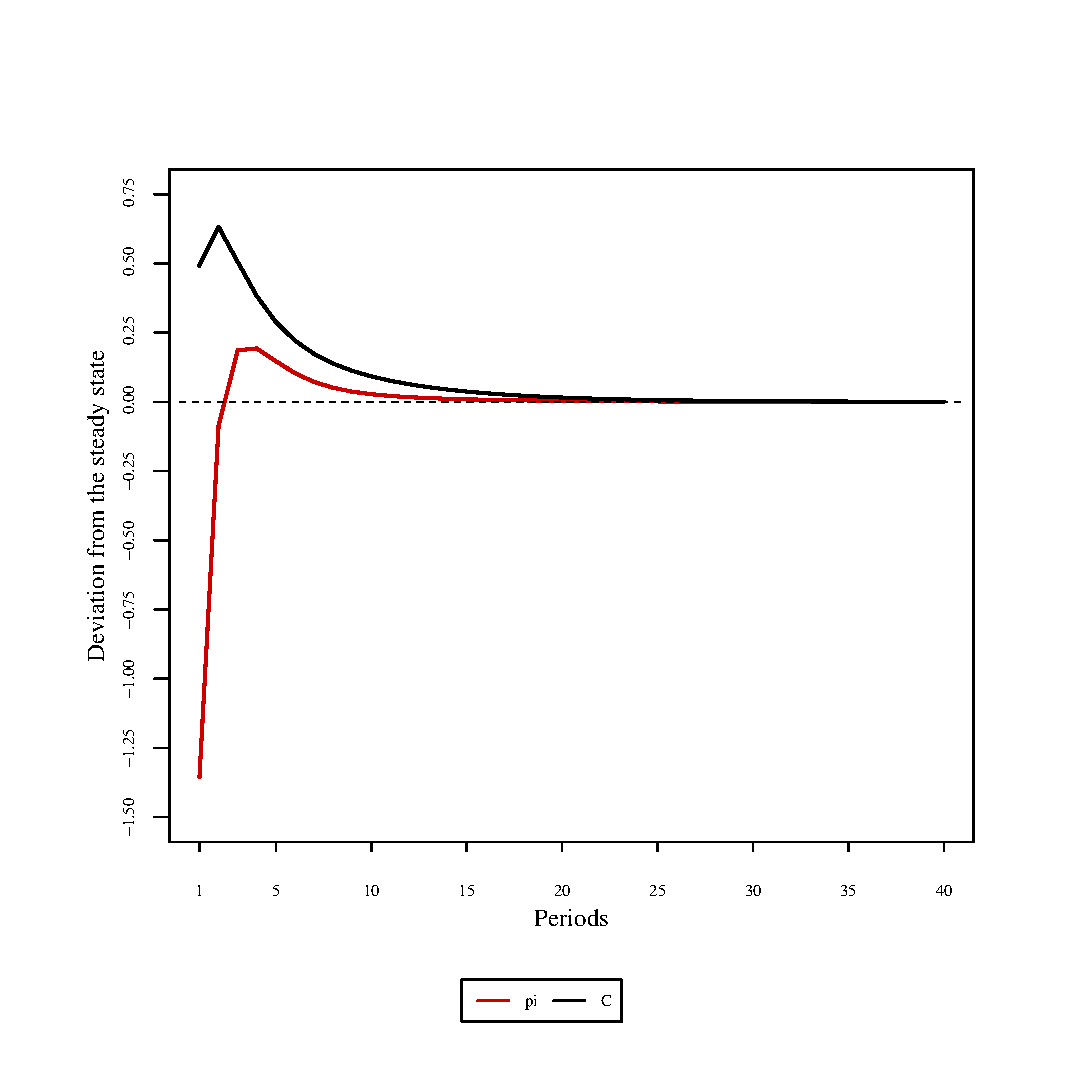
\includegraphics[width=0.99\textwidth, scale=0.55]{plots/plot_26.eps}
\caption{Impulse responses ($\pi, C$) to $\epsilon^{\mathrm{Z}}$ shock}
\end{minipage}
\begin{minipage}{0.5\textwidth}
\vspace*{-3em}
\centering
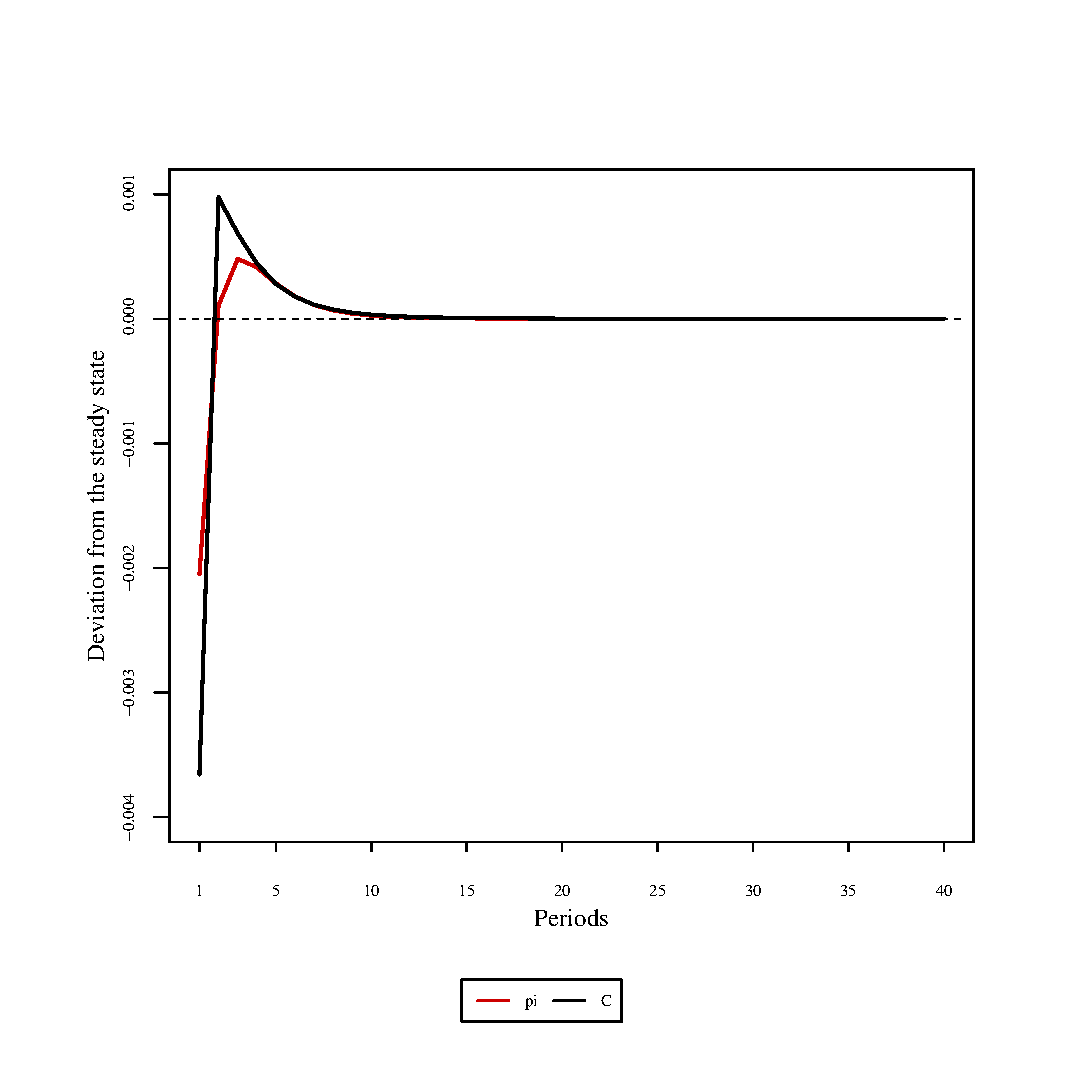
\includegraphics[width=0.99\textwidth, scale=0.55]{plots/plot_27.eps}
\caption{Impulse responses ($\pi, C$) to $\eta^{\mathrm{p}}$ shock}
\end{minipage}
\end{figure}

\begin{figure}[h]
\begin{minipage}{0.5\textwidth}
\vspace*{-3em}
\centering
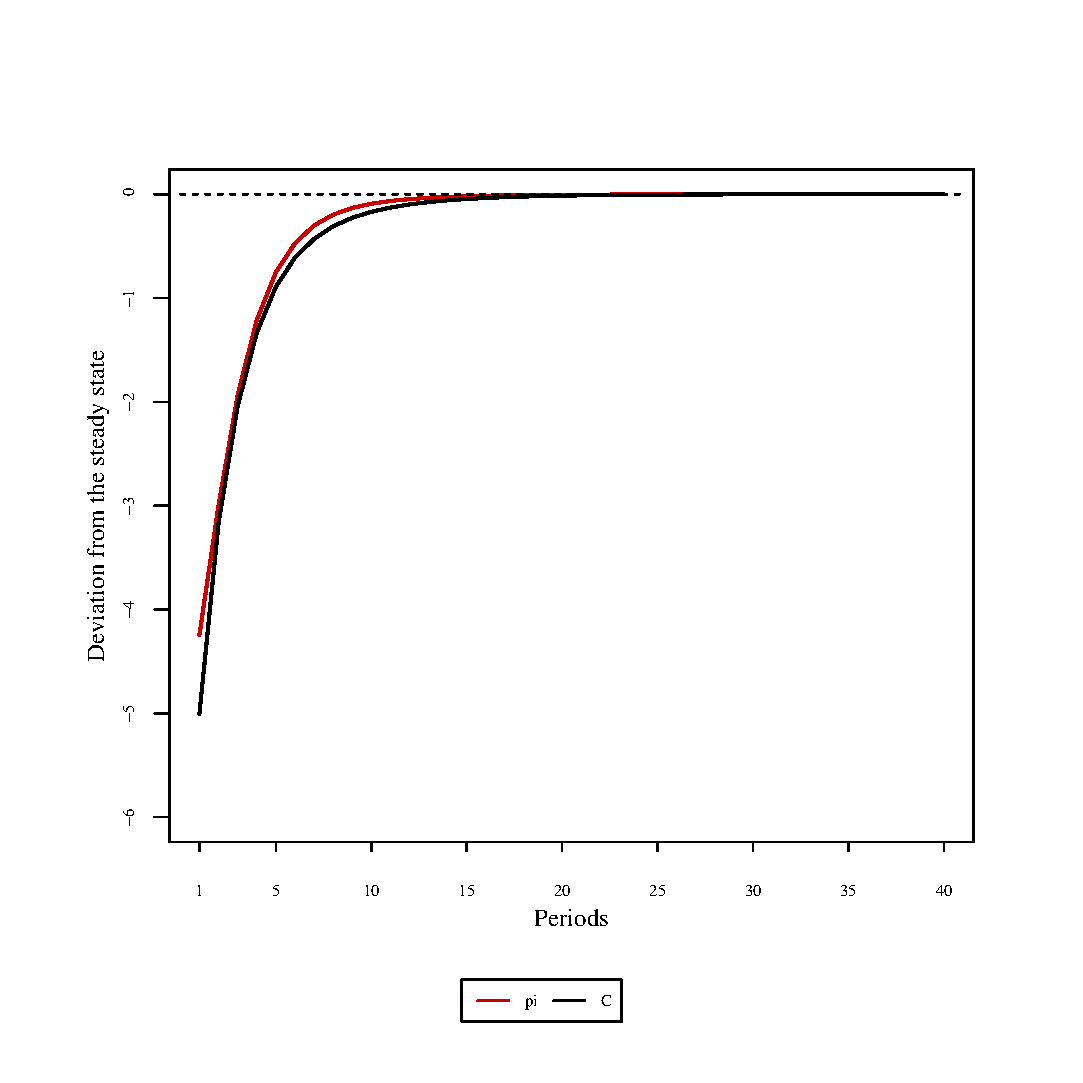
\includegraphics[width=0.99\textwidth, scale=0.55]{plots/plot_28.eps}
\caption{Impulse responses ($\pi, C$) to $\eta^{\mathrm{R}}$ shock}
\end{minipage}
\begin{minipage}{0.5\textwidth}
\vspace*{-3em}
\centering
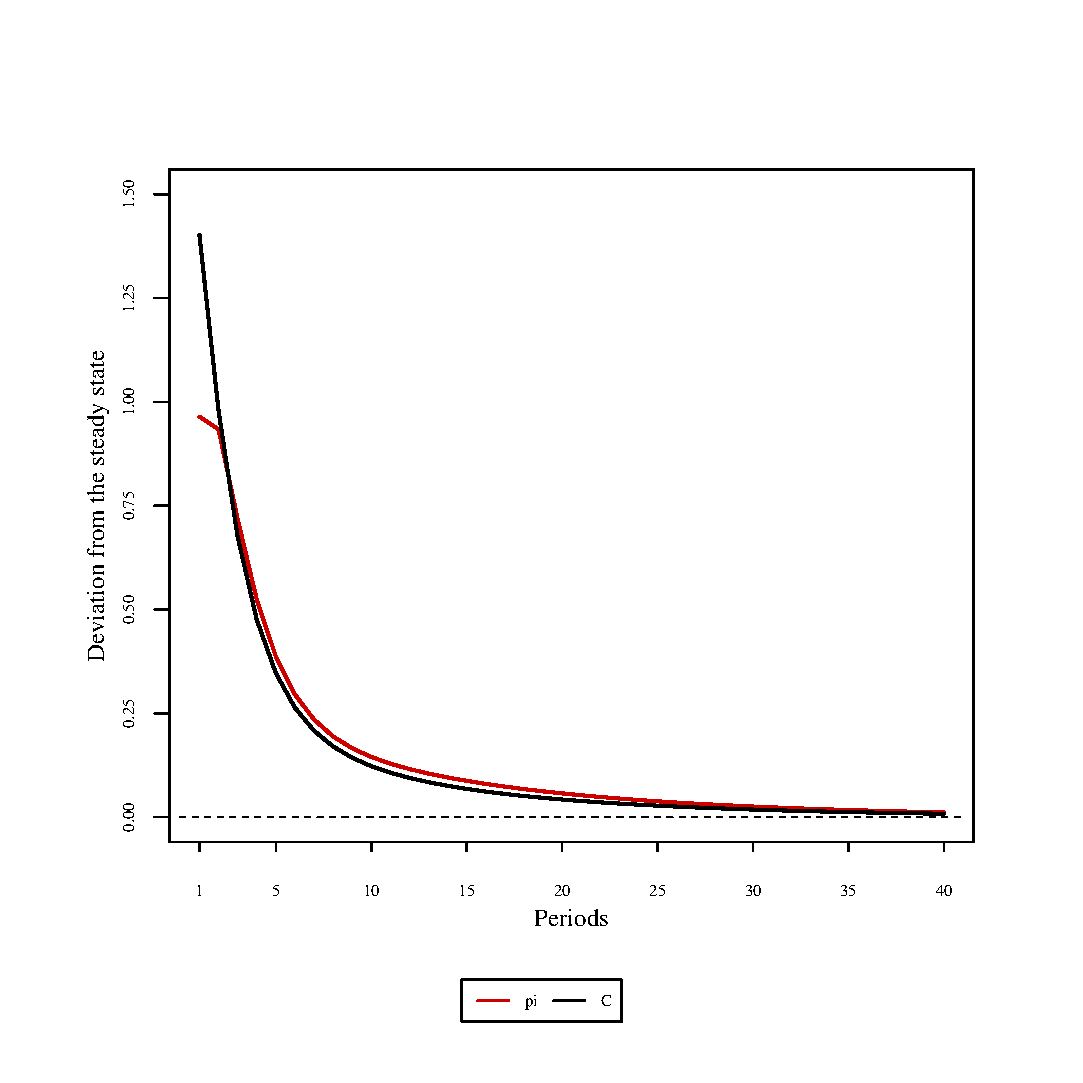
\includegraphics[width=0.99\textwidth, scale=0.55]{plots/plot_29.eps}
\caption{Impulse responses ($\pi, C$) to $\eta^{\pi}$ shock}
\end{minipage}
\end{figure}

\pagebreak

\begin{figure}[h]
\centering
\begin{minipage}{0.5\textwidth}
\vspace*{-3em}
\centering
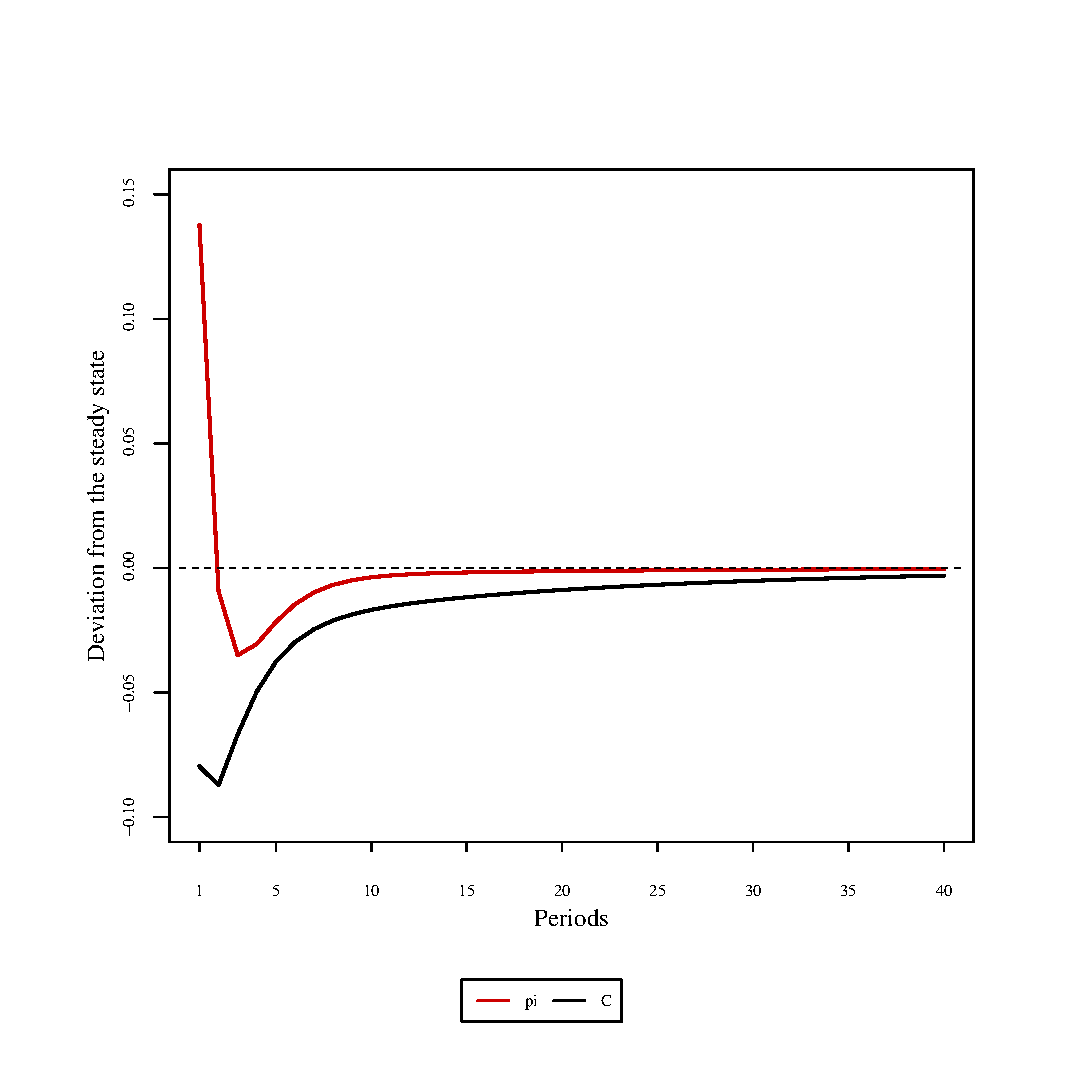
\includegraphics[width=0.99\textwidth, scale=0.55]{plots/plot_30.eps}
\caption{Impulse responses ($\pi, C$) to $\eta^{\mathrm{G}}$ shock}
\end{minipage}
\end{figure}
